\documentclass[conference]{IEEEtran}
\IEEEoverridecommandlockouts
% The preceding line is only needed to identify funding in the first footnote. If that is unneeded, please comment it out.
\usepackage{cite}
\usepackage{amsmath,amssymb,amsfonts}
\usepackage[hidelinks]{hyperref}
\usepackage{algorithmic}
\usepackage{graphicx}
\usepackage{booktabs}
\usepackage{textcomp}
\usepackage{xcolor}
\def\BibTeX{{\rm B\kern-.05em{\sc i\kern-.025em b}\kern-.08em
    T\kern-.1667em\lower.7ex\hbox{E}\kern-.125emX}}
\begin{document}


\title{Composition of concrete and its influence on compressive strength\\
%{\footnotesize \textsuperscript{*}Note: Sub-titles are not captured in Xplore and
%should not be used}
%\thanks{Identify applicable funding agency here. If none, delete this.}
}

\author{\IEEEauthorblockN{Filipe P. de Farias}
\IEEEauthorblockA{\textit{Department of Teleinformatics Engineering} \\
\textit{Federal University of Ceará}\\
Fortaleza, Brazil \\
filipepfarias@fisica.ufc.br}
\and
\IEEEauthorblockN{Yvo J. M. Sales}
\IEEEauthorblockA{\textit{Department of Teleinformatics Engineering} \\
\textit{Federal University of Ceará}\\
Fortaleza, Brazil \\
yvo@gtel.ufc.br}
}

\maketitle

\begin{abstract}
The compressive strength of a concrete is a important property since it impacts directly on its applications. The classical approach to obtain the compressive strength of a specific concrete mixture is to submit a sample to a test on a hydraulic press. However, it takes time to perform this type of test since it is necessary to wait the sample to cure. In this work, we try to find a regression model to accurately estimate the compressive strength of a concrete mixture from the concentration of its components.
\end{abstract}

\begin{IEEEkeywords}
Regression models, Concrete compressive strength, Machine-learning.
\end{IEEEkeywords}

\section{Introduction}
A material formed by aggregates bonded together by a fluid material that hardens over time has been used by humans for construction since many years ago\cite{b3}. Nowadays this material is known as concrete and it's widely used in the construction field. The aggregates used in the mixture of the concrete affect directly its compressive strength which highly impacts its applications. For instance, in general, the concrete for columns or beams needs to have a greater compressive strength than the one for pavement. On the previous work, we have made a statistical analysis on a dataset extracted from the UCI Machine Learning Repository (University of California, Irvine)\cite{b4} that collects information about the concentration of some aggregates used to form different mixtures of concretes. In this work, we try to find a regression model to estimate the relation between the concentration of those aggregates and the strength of the concrete mixture. The goal is that such model could be a good replacement to tests of samples on hydraulically press.

This work is divided as follows. A description of the data is given in Section~\ref{sec:data_description} resulted from the previous work with the addition of the regressor (concrete compressive strength). Section~\ref{sec:rm} brings a brief introduction to the regression models that will be used to fit the data. In the sequel, we present and discuss the results in Section~\ref{sec:results}. Finally, the conclusions and considerations are exposed in Section~\ref{sec:conclusions}.

% This works tries to predict this compressive strength and to classify when the concrete is proper to be applied in structures.  In the UCI database the concrete is tested with different components concentrations and different curing time (ages). 

\section{Data description}\label{sec:data_description}

The composition of each one of the $N$ concrete samples is given by the concentrations (kg/m\textsuperscript{3}) of $D$ components: Cement, Blast Furnace Slag, Fly Ash, Water, Superplasticizer, Coarse Aggregate and Fine Aggregate. The cement is what binds the elements of the concrete together. Indeed his technical name in the literature is \emph{binder} \cite{b5}. The other components as blast furnace slag and fly ash, the outcomes of another industrial process reused in the concrete mixture, they have the role of increase the chemical hardness of the concrete, i.e. in a microscopic level. The water is responsible for react with the cement resulting in the cement stone. The superplasticizer gives fluid characteristics to the concrete aiming to better fill the mold and decrease the use of water. The coarse and fine aggregates give some macroscopical mechanical resistance to the concrete but can reduce its compressive strength if bad applied. Their major role is to occupy the spaces in the mold reducing the use of cement. The output is the concrete compressive strength which is measure in the stress test where a force its applied to a sample using a hydraulic press. When the sample reaches rupture the pressure, force per area of the sample, is observed.

%Each sample has its Age (day) and the measured Concrete compressive strength (MPa), as described in Table~\ref{data_description_table}.

\begin{table}[htp]
\caption{Data description}
\begin{center}
  \begin{tabular}{@{} clc @{}}
    \toprule
    Label & Component & Unit \\ 
    \midrule
    $D_1$ & Cement & kg/m\textsuperscript{3} \\ 
    $D_2$ & Blast Furnace Slag & kg/m\textsuperscript{3} \\ 
    $D_3$ & Fly Ash & kg/m\textsuperscript{3} \\ 
    $D_4$ & Water & kg/m\textsuperscript{3} \\ 
    $D_5$ & Superplasticizer & kg/m\textsuperscript{3} \\ 
    $D_6$ & Coarse Aggregate & kg/m\textsuperscript{3} \\ 
    $D_7$ & Fine Aggregate & kg/m\textsuperscript{3} \\ 
    $D_8$ & Age & days \\ 
    ${\bf D_9}$ & {\bf Compressive strength} & {\bf MPa} \\ 
	\midrule
    Total & $N=$ 1030 samples&  \\ 
    \bottomrule
  \end{tabular}
\end{center}
\label{data_description_table}
\end{table}%

%The concrete was stratified into $L=3$ classes\cite{b1}. The concrete which is weak and not recommended for structures, the \emph{Non-standard}, was labeled with $L_1$ and has 295 samples in it. The concrete whose strength is in a range that can be applied to structures is classified as $L_2$, or \emph{Standard}, and has 525 samples. The high performance concrete $L_3$, \emph{High-strength} and has 210 samples.
The observations are the measured compressive strengths of each sample and, as the predictors $D_1 - D_7$, are continuous. The Age ($D_8$) of the concrete is extremely discrete. All the data was normalised, by centering at the mean and scaling by the standard deviation to avoid any of the methods to be sensitive to different scales. At Fig. \ref{histogram_biplot} we note the strongest positive correlation is between the strength and the cement component ($D_9 \times D_1$). Another important factors are the presence of the superplasticizer ($D_9 \times D_5$) and the age that represents the time of cure ($D_9 \times D_8$). In all these components is noted a subtle correlation. And the most important fact that can be observed is the decrease of the necessity of water when the superplasticizer is used ($D_5 \times D_4$), which was its proposal in the first place.
\begin{figure}[htbp]
\centerline{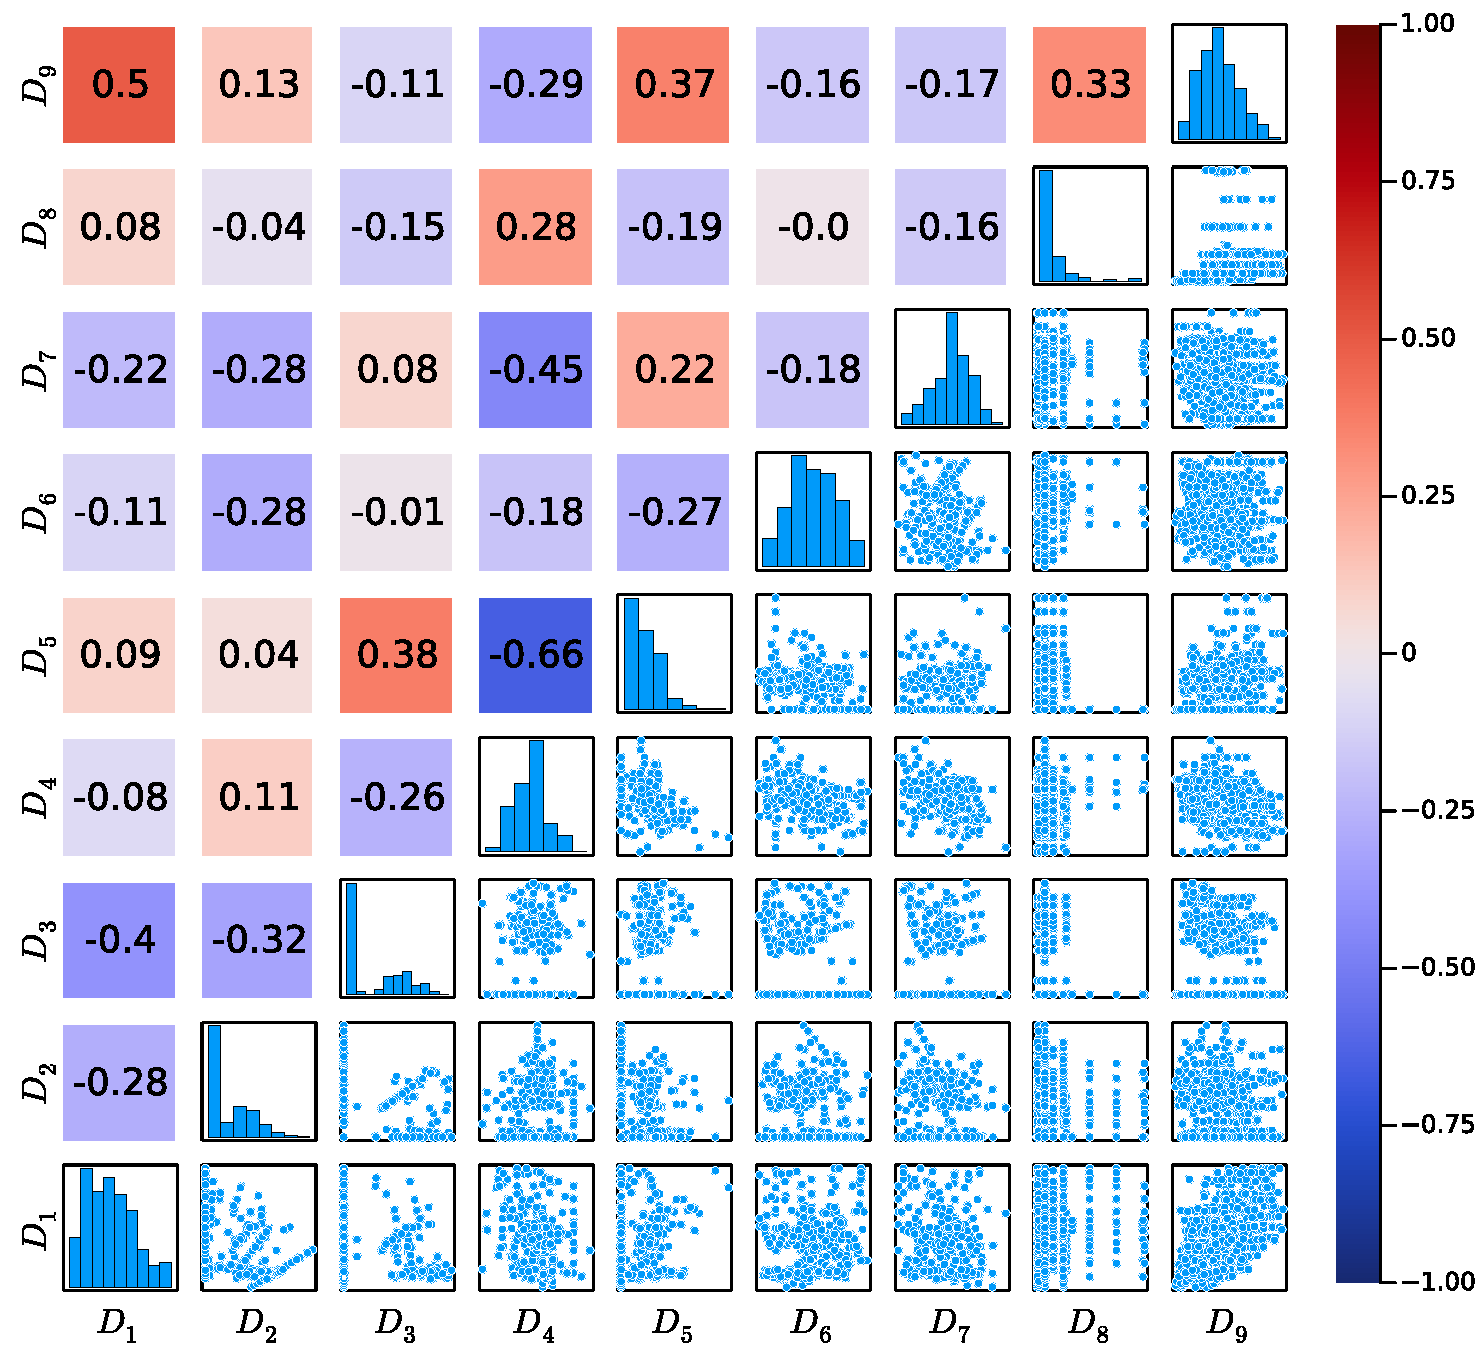
\includegraphics[width=\columnwidth]{../figures/correlation_predictors_outcomes}}
\caption{Pairwise scatter, correlation and histogram plots of each concrete component.}
\label{histogram_biplot}
\end{figure}

\section{Regression models}\label{sec:rm}

Regression models try to find relations between the \emph{independent variables} and the \emph{dependent variables}, which are named, respectively, predictors and outcomes in this work. These relations can occur in different forms. The simplest one is the linear relationship, which is when the curve predictors \textit{vs} outcomes, in the case that both are one-dimensional, forms a simple line and, in the general case, a hyperplane. In what follows, we formulate the \emph{Linear regression}, which is a subclass of regressions dedicated to find a linear model to explain the relation between the predictors and the outcomes. 


\subsection{Linear regression}

\begin{align} \label{eq:lm}   
  Y &= \begin{bmatrix} 
        \beta_0 & \boldsymbol{\beta}^\top 
       \end{bmatrix} 
       \begin{bmatrix} 
        \mathbf{1} \\ X 
      \end{bmatrix} + \varepsilon
\end{align} 

This method tries to find the linear regression between the predictors and outcomes by fitting a line with linear coefficient $\boldsymbol{\beta}$ and angular coefficient $\boldsymbol{\beta}$, defined in Eq.~(\ref{eq:lm}), through the data. $\boldsymbol{\beta}$ is the size such as the number of predictors in $X$, in the way we can define the vector $\boldsymbol{\beta} = [\beta_0, ..., \beta_D]^\top$. Wrapping up $[\beta_0 \ \boldsymbol{\beta}]^\top$ is a $1\times (D+1)$, $\mathbf{x} = [\mathbf{1} \ X]^\top$ is a $(N+1)\times D$ matrix and $Y$ is a $N\times 1$ matrix. For limitations on the implementation, it was adopted the label $D_9$ for the outcome, then the dimension $D$ of the matrices must be considered without the outcome component, that is 8 components.

The fitting, i.e. finding the values for each of the linear and angular coefficients, is done by minimising a cost function that can take different forms. Each cost function yields to different optimal parameters and two of them are described in the following, the \emph{Ordinary least squares} and \emph{L\textsubscript{2}-penalized least squares}. An interesting fact to observe is when the predictors correlates with the outcome, we can observe the error will be small. This is because the correlation evaluates linear variations between the variables as such as the linear regression.

The \emph{Ordinary least squares} defines the cost function to find the optimal parameters for Eq.~(\ref{eq:lm}) as

\begin{equation}\label{eq:cf_ols}
  L(\mathbf{y}, \boldsymbol{\beta}) =\sum_{i=1}^{n}\left(y_{i}-\beta_{0}-\sum_{j=1}^{p} \beta_{j} x_{i j}\right)^{2}.
\end{equation}
%
This cost function represents a quadratic distance between the model, i.e. the linear combination of the coefficients and the data. We have the minimal distance, we obtain the best model. This minimisation can be done by differentiating Eq. (\ref{eq:cf_ols}) w.r.t. the $\beta$'s giving the coefficients $\hat{\boldsymbol{\beta}}$ of the best model by
%
\[
\hat{\boldsymbol{\beta}} = (\mathbf{x}^\top\mathbf{x})^{-1}\mathbf{x}^\top Y.
\]

The \emph{L\textsubscript{2}-penalized least squares} modifies Eq.~(\ref{eq:cf_ols}) adding a term that penalize large values of the parameters, yielding to

\begin{equation}
  L(\mathbf{y}, \boldsymbol{\beta}) = \sum_{i=1}^{n}\left(y_{i}-\beta_{0}-\sum_{j=1}^{p} \beta_{j} x_{i j}\right)^{2}+\lambda \sum_{j=1}^{p} \beta_{j}^{2},
\end{equation}
%
where $\lambda$ is the penalisation coefficient, a tuning parameter. Different from ordinary least squares, we find $\lambda$ such the model will be the best one with \emph{cross-validation}. The values of the coefficients for a given $\lambda$ is 
%
\[
\hat{\boldsymbol{\beta}} = (\mathbf{x}^\top\mathbf{x} + \lambda)^{-1}\mathbf{x}^\top Y.
\]

\subsection{Partial least squares}

\section{Results} \label{sec:results}

\begin{figure}[htbp]
\centerline{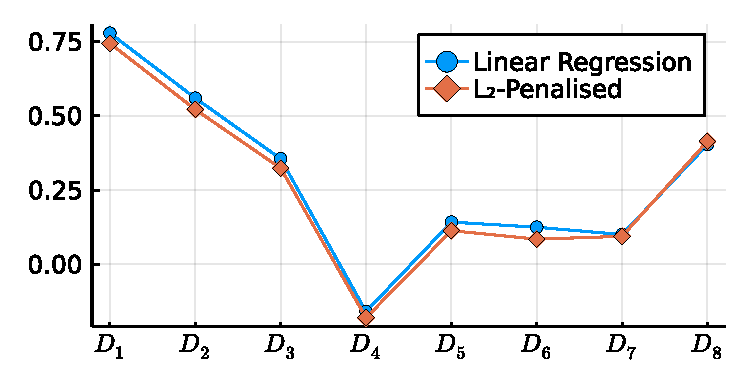
\includegraphics[width=\columnwidth]{../figures/fitted_params_70}}
\caption{Values of the weights of each predictor obtained after 30\%/70\% cross-validation strategy.}
%\label{histogram_biplot}
\end{figure}

\begin{figure}[htbp]
\centerline{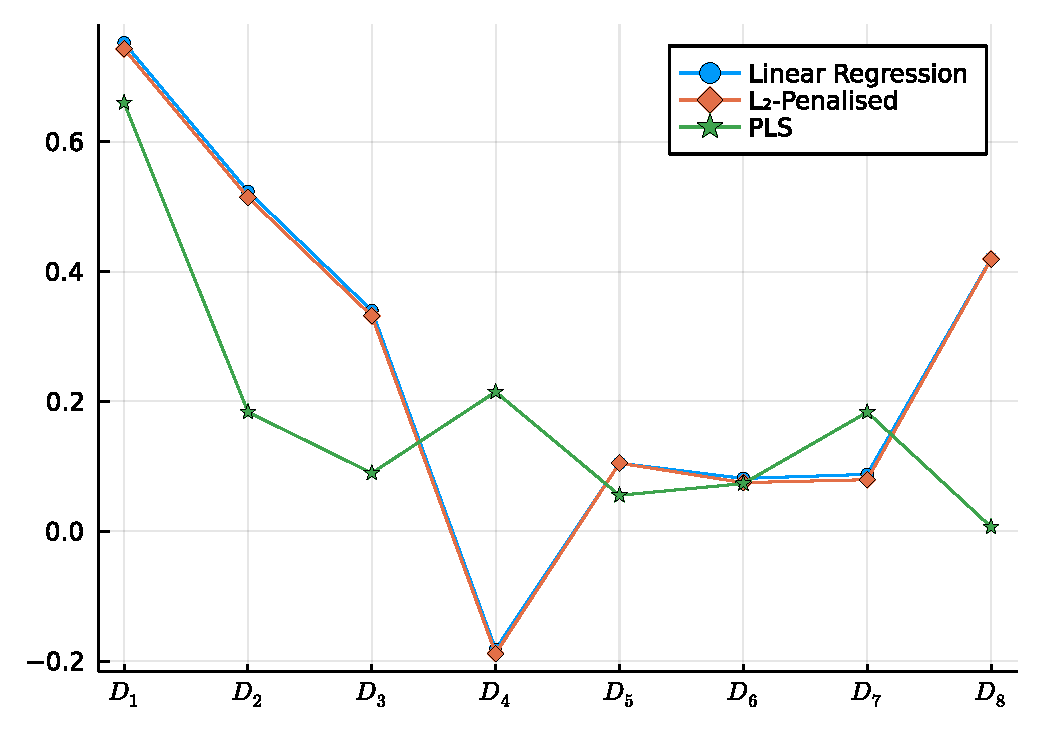
\includegraphics[width=\columnwidth]{../figures/fitted_params_kfolds}}
\caption{Values of the weights of each predictor obtained after $5$-fold cross-validation strategy.}%\label{histogram_biplot}
\end{figure}

\begin{table}[h!] 
\centering
  \caption{Ordinary Least Squares Regression Summary}
  \label{table:ols}
  \begin{tabular}{crr}
    \toprule
    {CV} & {RMSE} & {$R^2$} \\\hline
    70\% Train / 30\% Test & 0.614014 & 0.612271 \\
    1-st fold & 0.614187 & 0.634496 \\
    2-dn fold & 0.647336 & 0.597003 \\
    3-rd fold & 0.5952 & 0.599484 \\
    4-th fold & 0.686377 & 0.530463 \\
    5-th fold & \textbf{0.582266} & \textbf{0.661407} \\\bottomrule
  \end{tabular}
\end{table}


\begin{table}
\centering
  \caption{$L_2$-penalized Least Squares Regression Summary}
  \begin{tabular}{crr}
    \toprule
    {CV} & {RMSE} & {$R^2$} \\\hline
    70\% Train / 30\% Test & 0.599004 & 0.640309 \\
    1-st fold & 0.613885 & 0.634857 \\
    2-dn fold & 0.647344 & 0.596994 \\
    3-rd fold & 0.594722 & 0.600127 \\
    4-th fold & 0.68599 & 0.530993 \\
    5-th fold & \textbf{0.582357} & \textbf{0.661302} \\\bottomrule
  \end{tabular}
\end{table}

\begin{table}[t]
\centering
  \caption{Partial Least Squares Regression Summary}
  \label{table:pls}
  \begin{tabular}{crr}
    \toprule
    {CV} & {RMSE} & {$R^2$} \\\hline
    70\% Train / 30\% Test & 0.599264 & 0.639996 \\
    1-st fold & 0.614106 & 0.634593 \\
    2-dn fold & 0.646593 & 0.597928 \\
    3-rd fold & 0.594709 & 0.600143 \\
    4-th fold & 0.6859 & 0.531116 \\
    5-th fold & \textbf{0.58221} & \textbf{0.661472} \\\bottomrule
  \end{tabular}
\end{table}


\section{Conclusions}\label{sec:conclusions}

The database of concrete is not easy to analyse if there is no previous knowledge about the problem of the components mixture. In none of the analysis the data have been shown as separable on the initially determined classes. The next step is to try to perform regression to model the compressive strength itself before trying to classify the samples. in the literature \cite{b6} is more common an analysis of the concrete data stratified by the Age, what was not done in this work and maybe the cause of poor correlations.

\begin{thebibliography}{00}
\bibitem{b1} ACI Manual of Concrete Practice 2000, Part 1: Materials and General Properties of Concrete.  American Concrete Institute.  Farmington Hills, MI.
\bibitem{b2} Tibshirani, Robert, et al. The Elements of  Statistical Learning:  Data Mining, Inference, and Prediction. Germany, Springer New York, 2009.
\bibitem{b3} Mindess, S., and Young, J.F. Concrete. Prentice-Hall, Inc., Englewood Cliffs, NJ, 1981.
\bibitem{b4} I-Cheng Yeh, ``Modeling of strength of high performance concrete using artificial neural networks," Cement and Concrete Research, Vol. 28, No. 12, pp. 1797-1808 (1998)
\bibitem{b6} I-Cheng Yeh, ``Prediction of Strength of Fly Ash and Slag Concrete By The Use of Artificial Neural Networks," Journal of the Chinese Institute of Civil and Hydraulic Engineering, Vol. 15, No. 4, pp. 659-663 (2003). 
\bibitem{b5} Khasanov, Irmuhamedova, et al, ``Theoretical foundations of the structure formation of cement stone
and concrete," IOP Conf. Series: Materials Science and Engineering 869 (2020)
\end{thebibliography}
\end{document}